\documentclass[a4paper,12pt]{article}

% ---------- FONT & LANGUAGE ----------
\usepackage{fontspec}
\usepackage{polyglossia}
\usepackage{caption}
\usepackage{float}
\usepackage{booktabs}
\usepackage{multirow}
\usepackage{array}
\usepackage{hyperref}
\usepackage{tikz}
\usepackage{pgfplots}
\usepackage{subcaption}
\usepackage{enumitem}
\usepackage{amsmath}
\usepackage{amsfonts}
\usepackage{amssymb}
\usepackage{graphicx}
\usepackage{listings}
\usepackage{xcolor}
\usepackage{geometry}
\geometry{margin=1in}

\setmainlanguage{greek}
\setotherlanguage{english}

% Γραμματοσειρές
\newfontfamily\greekfont{Times New Roman}[Script=Greek, Scale=1.0]
\newfontfamily\englishfont{Times New Roman}[Script=Latin, Scale=1.0]

% Μονοσύστημα γραμματοσειρά για ελληνικά και κώδικα
\newfontfamily\greekfonttt{Consolas}[Scale=MatchLowercase]
\newfontfamily\englishfonttt{Consolas}[Scale=MatchLowercase]

\hypersetup{
	colorlinks=true,
	linkcolor=black,
	urlcolor=black,
}

% ---------- CODE STYLE ----------
\definecolor{codegreen}{rgb}{0,0.6,0}
\definecolor{codegray}{rgb}{0.5,0.5,0.5}
\definecolor{codepurple}{rgb}{0.58,0,0.82}
\definecolor{backcolour}{rgb}{0.95,0.95,0.92}

\lstdefinestyle{mystyle}{
	backgroundcolor=\color{backcolour},
	commentstyle=\color{codegreen},
	keywordstyle=\color{magenta},
	numberstyle=\tiny\color{codegray},
	stringstyle=\color{codepurple},
	basicstyle=\ttfamily\footnotesize,
	breakatwhitespace=false,
	breaklines=true,
	captionpos=b,
	keepspaces=true,
	numbers=left,
	numbersep=5pt,
	showspaces=false,
	showstringspaces=false,
	showtabs=false,
	tabsize=4,
	language=C
}

\lstset{style=mystyle}

\title{Δεύτερο Σετ Ασκήσεων\\PART II: “BSTs (Balanced Search Trees) \&\& HASHING” \\ Δομές Δεδομένων 2025-2026}
\author{
	Ανδριόπουλος Ιωάννης ΑΜ: 1115519\\
	Καραπατάκης Ευθύμιος ΑΜ: 1115521\\
	Χριστοπούλου Αγγελική ΑΜ: 1115471
}

\begin{document}
	
	\maketitle
	\newpage
	\tableofcontents
	\newpage
	
	\section{Εκφώνηση Εργασίας}
	
	Με τον κατάλληλο ορισμό δομών (structs) / κλάσεων (classes) και συναρτήσεων (functions) / μεθόδων
	(methods), να υλοποιήσετε μια εφαρμογή (σε γλώσσα C, C++ ή Java) που θα επεξεργάζεται τα
	δεδομένα του αρχείου “dataset effects-of-covid-19-on-trade-at-15-december-2021-provisional.csv”.
	Θυμίζουμε ξανά ότι κάθε γραμμή του αρχείου αυτού αντιστοιχεί σε μία ημέρα μετρήσεων.
	
	\subsection{Ζητούμενα}
	\begin{itemize}
		\item[(Α)] Η εφαρμογή διαβάζει αρχικά το αρχείο και δημιουργεί ένα Δένδρο BST (Ισοζυγισμένο Δυαδικό
		Δέντρο ) στο οποίο κάθε κόμβος του διατηρεί την εγγραφή (Date, Cumulative της ημέρας αυτής).
		Το BST διατάσσεται ως προς την ΗΜΕΡΟΜΗΝΙΑ (Date) και υλοποιείται με δυναμική διαχείριση
		μνήμης. Προτιμότερες επιλογές AVL, red-black, (2,4) δέντρα. Μετά την δημιουργία του BST η
		εφαρμογή εμφανίζει ένα μενού με τις ακόλουθες επιλογές:
		\begin{enumerate}
			\item Απεικόνιση του BST με ενδο-διατεταγμένη διάσχιση. Κάθε απεικόνιση θα πρέπει να περιέχει
			μια επικεφαλίδα με τους τίτλους των στοιχείων των εγγραφών που απεικονίζονται.
			\item Αναζήτηση της τιμής Cumulative βάσει ΗΜΕΡΟΜΗΝΙΑΣ (Date) που θα δίνεται από το
			χρήστη.
			\item Τροποποίηση του περιεχομένου του πεδίου Cumulative που αντιστοιχεί σε συγκεκριμένη
			ΗΜΕΡΟΜΗΝΙΑ (Date).
			\item Διαγραφή μιας εγγραφής που αντιστοιχεί σε συγκεκριμένη ΗΜΕΡΟΜΗΝΙΑ (Date).
			\item Έξοδος από την εφαρμογή.
		\end{enumerate}
		\item[(Β)] Τροποποιήστε κατάλληλα τον κώδικα του (Α), ώστε το αρχείο να διαβάζεται στο BST με βάση
		την τιμή του πεδίου Cumulative. Το BST διατάσσεται ως προς την τιμή Cumulative ανά
		ΗΜΕΡΟΜΗΝΙΑ (Date) και υλοποιείται με δυναμική διαχείριση μνήμης. Μετά την δημιουργία του
		BST η εφαρμογή εμφανίζει ένα μενού με τις ακόλουθες επιλογές:
		\begin{enumerate}
			\item Εύρεση ΗΜΕΡΑΣ/ΗΜΕΡΩΝ με την ΕΛΑΧΙΣΤΗ ΤΙΜΗ Cumulative.
			\item Εύρεση ΗΜΕΡΑΣ/ΗΜΕΡΩΝ με τη ΜΕΓΙΣΤΗ ΤΙΜΗ Cumulative.
		\end{enumerate}
		\item[(Γ)] Υλοποιήστε το (Α) κάνοντας χρήση HASHING με αλυσίδες, αντί BST. Η συνάρτηση
		κατακερματισμού θα υπολογίζεται ως το υπόλοιπο (modulo) της διαίρεσης του αθροίσματος των
		κωδικών ASCII των επιμέρους χαρακτήρων που απαρτίζουν την ΗΜΕΡΟΜΗΝΙΑ με ένα περιττό
		αριθμό m που συμβολίζει το πλήθος των κάδων (buckets). Π.χ. για ΗΜΕΡΟΜΗΝΙΑ=”
		15/12/2021” και m=11, ισχύει:\\
		\\
		Hash("15/12/2021")= [ASCII(‘1’)+ ASCII(‘5’)+ ASCII(‘/’)+ ASCII(‘1’)+ ASCII(‘2’)+ ASCII(‘/’)+
		ASCII(‘2’)+ ASCII(‘0’)+ ASCII(‘2’)+ ASCII(‘1’)] mod 11.\\
		\\
		Το πρόγραμμα θα εμφανίζει ένα μενού με τις ακόλουθες επιλογές:\\
		\begin{enumerate}
			\item Αναζήτηση Τιμής Cumulative βάσει της ΗΜΕΡΟΜΗΝΙΑΣ που θα δίνεται από το χρήστη.
			\item Τροποποίηση των στοιχείων εγγραφής βάσει ΗΜΕΡΟΜΗΝΙΑΣ που θα δίνεται από το χρήστη. Η τροποποίηση προφανώς αφορά ΜΟΝΟ το πεδίο Cumulative.
			\item Διαγραφή μιας εγγραφής από τον πίνακα κατακερματισμού βάσει ΗΜΕΡΟΜΗΝΙΑΣ που θα δίνεται από το χρήστη.
			\item Έξοδος από την εφαρμογή.
		\end{enumerate}
		Ενοποιήστε τα (Α), (Β) και (Γ) σε ένα πρόγραμμα στο οποίο ο χρήστης θα ερωτάται αν θέλει τη φόρτωση
		του αρχείου σε ένα BST ή σε μία δομή Hashing με αλυσίδες και στην περίπτωση που ο χρήστης επιλέξει
		το πρώτο να μπορεί εν συνεχεία να επιλέξει αν η φόρτωση στο BST θα γίνει με βάση την ΗΜΕΡΟΜΗΝΙΑ
		ή την τιμή Cumulative ανά ημέρα.
	\end{itemize} 
	
	\newpage
	
\section{Εισαγωγή}

Αυτό το project αναλύει το dataset \textit{Effects of COVID-19 on Trade (2015–2021)} το οποίο περιέχει 111.438 εγγραφές. Κάθε εγγραφή περιέχει:

\begin{center}
	Direction, Year, Date, Weekday, Country, Commodity, Transport Mode, Measure, Value, Cumulative
\end{center}

Στόχος είναι η υλοποίηση και η σύγκριση κλασικών αλγορίθμων ταξινόμησης και αναζήτησης χρησιμοποιώντας αυτό το πραγματικό σύνολο δεδομένων.

\section{Περιγραφή Δεδομένων}

Το dataset περιέχει στατιστικά στοιχεία εμπορίου που σχετίζονται με εισαγωγές, εξαγωγές και επανεισαγωγές. Κάθε εγγραφή περιλαμβάνει αριθμητικά πεδία όπως:

\begin{itemize}
	\item \textbf{Value}: Εμπορική αξία σε δολάρια ή τόνους
	\item \textbf{Cumulative}: Αθροιστική εμπορική αξία σε δολάρια ή τόνους
	\item \textbf{Date}: Ημερομηνία στην μορφή ΗΗ/ΜΜ/ΕΕΕΕ
\end{itemize}

\begin{table}[H]
	\centering
	\begin{tabular}{|l|l|l|}
		\hline
		\textbf{Πεδίο} & \textbf{Τύπος} & \textbf{Περιγραφή} \\
		\hline
		Direction & String & imports, exports, reimports \\
		Year & Integer & 2015-2021 \\
		Date & Date & dd/mm/yyyy \\
		Weekday & String & Monday-Sunday \\
		Country & String & Χώρα εμπορικού εταίρου \\
		Commodity & String & Κατηγορία προϊόντος \\
		Transport\_Mode & String & sea, air, κλπ. \\
		Measure & String & \$ ή Tonnes \\
		Value & Long Integer & Εμπορική αξία \\
		Cumulative & Long Integer & Αθροιστική αξία \\
		\hline
	\end{tabular}
	\caption{Δομή του Dataset}
\end{table}

\newpage

\section{Επισκόποιηση Υλοποιήσης}

Το σύστημα υλοποιήθηκε σε C και περιλαμβάνει 2 βασικές ενότητες:\\
\begin{itemize}
	\item Δημιουργία Δέντρου BST
	\item Δημιουργία Hashing με αλυσίδες
\end{itemize}

\begin{lstlisting}[caption=Δομή Record στη C]
	typedef struct {
		char direction[DIRECTION];
		char year[YEAR];
		char date[DATE];
		char weekday[WEEKDAY];
		char country[MAX_STR];
		char commodity[MAX_STR];
		char transport_mode[MAX_STR];
		char measure[MAX_STR];
		long long value;
		long long cumulative;
	} Record;
\end{lstlisting}

\subsection{Φόρτωση Δεδομένων}

\begin{lstlisting}[caption=Φόρτωση CSV]
	int load_csv(const char *filename, Record *data) {
		FILE *fptr = fopen(filename, "r");
		if(!fptr) {
			printf("[ERROR] No file %s found.\n", filename);
			return -1;
		}
		
		char line[512]; //temp info saver
		int count = 0;
		
		fgets(line, sizeof(line), fptr);
		
		while (fgets(line, sizeof(line), fptr) && count < MAX_ROWS) {
			line[strcspn(line, "\r\n")] = 0;
			
			char *temp;
			Record r;
			memset(&r, 0, sizeof(r));
			
			temp = strtok(line, ",");
			if(!temp) continue;
			strncpy(r.direction, temp, DIRECTION-1);
			
			temp = strtok(NULL, ",");
			if(!temp) continue;
			strncpy(r.year, temp, YEAR-1);
			
			temp = strtok(NULL, ",");
			if(!temp) continue;
			strncpy(r.date, temp, DATE-1);
			
			temp = strtok(NULL, ",");
			if(!temp) continue;
			strncpy(r.weekday, temp, sizeof(r.weekday) - 1);
			
			temp = strtok(NULL, ",");
			if(!temp) continue;
			strncpy(r.country, temp, sizeof(r.country) - 1);
			
			temp = strtok(NULL, ",");
			if(!temp) continue;
			strncpy(r.commodity, temp, sizeof(r.commodity) - 1);
			
			temp = strtok(NULL, ",");
			if(!temp) continue;
			strncpy(r.transport_mode, temp, sizeof(r.transport_mode) - 1);
			
			temp = strtok(NULL, ",");
			if(!temp) continue;
			strncpy(r.measure, temp, sizeof(r.measure) - 1);
			
			temp = strtok(NULL, ",");
			if(!temp) continue;
			r.value = atoll(temp);
			
			temp = strtok(NULL, ",");
			if(!temp) continue;
			r.cumulative = atoll(temp);
			
			data[count++] = r;
		}
		
		fclose(fptr);
		return count;
	}
\end{lstlisting}

\section{Άσκηση (Α): Υλοποιήση Εφαρμογής με BST, με βάση DATE}
\subsection{Περιγραφή}
Υλοποιήθηκε με Δέντρο AVL. Κάθε κόμβος του δέντρου αποθηκεύει έναν δείκτη στον δυναμικά δεσμευμένο πίνακα που περιέχει τα δεδομένα του CSV.\\
\begin{lstlisting}[caption={Δομή κόμβου}]
	typedef struct Node {
		Record* record;
		struct Node* left;
		struct Node* right;
		int height;
	} Node;
\end{lstlisting}
1.Για το πρώτο ερώτημα, το δέντρο εμφανίζεται με in-order Traversal.\\
\begin{lstlisting}[caption={Συνάρτηση inorder}]
	void inorder(Node* root) {
		if(!root) return;
		
		inorder(root->left);
		
		printf("Date: %-d/%d/%d \t Cumulative: %lld\n", 
		root->record->date[0], root->record->date[1], root->record->date[2],
		root->record->cumulative);
		
		inorder(root->right);
	}
\end{lstlisting}
2.Για το δεύτερο ερώτημα, χρησιμοποιήται κλασική Δυαδική Αναζήτηση. Η δοθείσα ημερομηνία συγκρίνεται με τον τρέχοντα κόμβο. Αν είναι μικρότερη, η αναζήτηση συνεχίζεται στο αριστερό παιδί. Αν είναι μεγαλύτερη, στο δεξί.\\
\begin{lstlisting}[caption={Συνάρτηση search}]
	Node* search(Node* root, int date[3]) {
		if(!root) return NULL;
		
		int cmp = compareDates(date, root->record->date);
		
		if(cmp == 0) return root;
		
		if(cmp < 0) return search(root->left, date);
		
		return search(root->right, date);
	}
\end{lstlisting}
3.Για το τρίτο ερώτημα, χρησιμοποιήται η συνάρτηση search του προηγούμενου ερωτήματος και όταν βρεθεί ο κόμβος, ο αλγόριθμος τον αντικαθιστά με την νέα τιμή.\\
\begin{lstlisting}[caption={Συνάρτηση modify}]
	Node* modify(Node* root, int date[3], long long value) {
		Node* node = search(root, date);
		
		if (node) {
			node->record->cumulative = value;
		} else {
			printf("Date not found.\n");
		}
		
		return root;
	}
\end{lstlisting}
4.Για το τέταρτο ερώτημα, χρησιμοποιήται η συνάρτηση search του προηγούμενου ερωτήματος και αν βρεθεί διαγράφεται. Αν έχει δύο παιδιά, δεν κόβονται οι συνδέσεις του δέντρου. Αντίθετα, βρίσκεται ο "in-order διάδοχος", ανταλλάσσονται οι δείκτες Record* (swapNodes), και διαγράφεται αναδρομικά ο διπλότυπος κόμβος.Τέλος, κατά την επιστροφή της αναδρομής, καλείται η balance για να εξασφαλιστεί ότι το δέντρο παραμένει ισοζυγισμένο.\\
\begin{lstlisting}[caption={Συνάρτηση deleteNode}]
	Node* deleteNode(Node* root, int date[3]) {
		if(!root) {
			printf("No nodes present.\n");
			return NULL;
		}
		
		int cmp = compareDates(date, root->record->date);
		
		if (cmp < 0) {
			root->left = deleteNode(root->left, date);
		} else if (cmp > 0) {
			root->right = deleteNode(root->right, date);
		} else {
			if(!root->left || !root->right) {
				Node* temp = root->left ? root->left : root->right;
				free(root);
				return temp;
			}
			
			Node* junior = minNode(root->right);
			swapNodes(root, junior);
			root->right = deleteNode(root->right, junior->record->date);
		}
		
		return balance(root);
	}
\end{lstlisting}
5.Για το πέμπτο ερώτημα, απελευθερώνεται η μνήμη του δυναμικού πίνακα δεδομένων (free(original)) αποτρέποντας διαρροές μνήμης (memory leaks) και το πρόγραμμα τερματίζει.

\section{Άσκηση (Β): Υλοποιήση Εφαρμογής με BST, με βάση\\CUMULATIVE}
\subsection{Περιγραφή}
Το Δέντρο AVL διατάσσεται με βάση την τιμή Cumulative. πειδή στα δεδομένα είναι βέβαιο ότι πολλές διαφορετικές ημέρες θα έχουν ακριβώς την ίδια τιμή Cumulative, η κλασική δομή του κόμβου επεκτάθηκε.\\
Αντί να δημιουργούνται περιττοί κόμβοι στο δέντρο που θα αλλοίωναν την ισορροπία του, ενσωματώθηκε μια απλά συνδεδεμένη λίστα (Singly Linked List) στο εσωτερικό κάθε κόμβου μέσω του δείκτη EqNode* equal.\\
Όταν η συνάρτηση insert εντοπίσει ότι το Cumulative της νέας εγγραφής ισούται με ένα ήδη υπάρχον (cmp == 0), δεν αλλοιώνει το δέντρο, αλλά καλεί την insertEqNode\_End η οποία προσθέτει την εγγραφή στο τέλος της λίστας του συγκεκριμένου κόμβου.\\
\begin{lstlisting}[caption={Δομή κόμβου}]
	typedef struct EqNode {
		Record* value;
		struct EqNode* next;
	} EqNode;
	
	typedef struct Node {
		Record* record;
		struct Node* left;
		struct Node* right;
		int height;
		
		EqNode* equal;
	} Node;
\end{lstlisting}
1. Για το πρώτο ερώτημα, αξιοποιείται η ιδιότητα του Δυαδικού Δέντρου Αναζήτησης ότι η ελάχιστη τιμή βρίσκεται στο αριστερότερο φύλλο. Η συνάρτηση findMin ξεκινά από τη ρίζα και μεταβαίνει διαρκώς στο αριστερό παιδί (root = root->left) μέχρι να συναντήσει NULL.\\
\begin{lstlisting}[caption={Συνάρτηση findMin}]
	Node* findMin(Node* root) {
		if(!root) return NULL;
		
		while(root->left) {
			root = root->left;
		}
		return root;
	}
\end{lstlisting}
Μόλις βρεθεί ο κόμβος, καλείται η printEqList η οποία διατρέχει τη συνδεδεμένη λίστα του κόμβου και εκτυπώνει όλες τις ημερομηνίες που μοιράζονται αυτή την ελάχιστη τιμή.\\
\begin{lstlisting}[caption={Συνάρτηση printDates\_Min}]
	void printDates_Min(Node* root) {
		Node* min = findMin(root);
		
		if (!min) {
			printf("The tree is empty.\n");
			return;
		}
		
		printf("The minimum Cumulative is: %lld", min->record->cumulative);
		printEqList(min);
	}
\end{lstlisting}
\begin{lstlisting}[caption={Συνάρτηση printEqList}]
	void printEqList(Node* node) {
		if(!node) return;
		
		Record* r = node->record;
		printf("Cumulative: %lld\n \tDate: %d/%d/%d\n", r->cumulative, r->date[0], 
		r->date[1], r->date[2]);
		
		EqNode* eq = node->equal;
		while(eq!= NULL) {
			r = eq->value;
			
			printf("Cumulative: %lld\n \tDate: %d/%d/%d\n", r->cumulative, r->date[0], 
			r->date[1], r->date[2]);
			eq = eq->next;
		}
	}
\end{lstlisting}
2. Για το δεύτερο ερώτημα, η συνάρτηση findMax διασχίζει το δέντρο ακολουθώντας συνεχώς τον δείκτη προς το δεξί παιδί (root = root->right) μέχρι να βρει τον τελευταίο κόμβο. Και πάλι χρησιμοποιείται η printEqList για να εκτυπωθούν όλες οι ισοβαθμούσες ημερομηνίες.\\
\begin{lstlisting}[caption={Συνάρτηση findMax}]
	Node* findMax(Node* root) {
		if(!root) return NULL;
		
		while(root->right) {
			root = root->right;
		}
		return root;
	}
\end{lstlisting}
\begin{lstlisting}[caption={Συνάρτηση printDates\_Max}]
	void printDates_Max(Node* root) {
		Node* max = findMax(root);
		
		if (!max) {
			printf("The tree is empty.\n");
			return;
		}
		
		printf("The maximum Cumulative is: %lld\n", max->record->cumulative);
		printEqList(max);
	}
\end{lstlisting}

\section{Άσκηση (Γ): Υλοποιήση Εφαρμογής με Hashing με αλυσίδες, με βάση DATE}
\subsection{Περιγραφή}
Υλοποιήθηκε με Hash Table χρησιμοποιώντας την μέθοδο αλυσίδων για την αντιμετώπιση των συγκρούσεων.\\
Η δομή HashMap αποτελείται από έναν πίνακα δεικτών μεγέθους m.\\
\begin{lstlisting}[caption={Δομή HashMap}]
	typedef struct {
		Node **buckets;
		int m;
		int totalRecords;
	}HashMap;
\end{lstlisting}
Διατηρείται η ίδια αποδοτική διαχείριση μνήμης με τα προηγούμενα ερωτήματα: Κάθε κόμβος της αλυσίδας δεν αντιγράφει τα δεδομένα, αλλά περιέχει απλώς έναν δείκτη προς τον κεντρικό πίνακα original.\\
Η συνάρτηση hashing υπολογίζει το άθροισμα των ASCII κωδικών των χαρακτήρων του αλφαριθμητικού της ημερομηνίας. Το τελικό index (κάδος) προκύπτει από το υπόλοιπο της διαίρεσης αυτού του αθροίσματος με το μέγεθος του πίνακα $m$: $Index = \left( \sum_{i} ASCII(Date[i]) \right) \pmod m$\\
Για την αντιμετώπιση συγκρούσεων όταν μια εγγραφή πρέπει να μπει σε έναν κάδο, ο νέος κόμβος εισάγεται πάντα στην αρχή (head) της συνδεδεμένης λίστας (newNode->next = map->buckets[index]).\\
1. Για το πρώτο ερώτημα, υπολογίζεται το index της δοθείσας ημερομηνίας μέσω της hash\_date. Στη συνέχεια, ο αλγόριθμος διασχίζει μόνο τη συνδεδεμένη λίστα του συγκεκριμένου κάδου, συγκρίνοντας τα strings (strcmp). Επειδή υπάρχουν διπλότυπες ημερομηνίες, η αναζήτηση δεν σταματάει στο πρώτο ταίριασμα, αλλά συνεχίζει για να εμφανίσει όλες τις σχετικές εγγραφές.\\
\begin{lstlisting}[caption={Συνάρτηση hash\_date}]
	int hash_date(char* date, int m) {
		unsigned long sum = 0;
		for(int i = 0; i < DATE-1; i ++) {
			sum += date[i];
		}
		return (int)(sum % (unsigned long)m);
	}
\end{lstlisting}
\begin{lstlisting}[caption={Συνάρτηση searchByDate}]
	int searchByDate(HashMap* map, char* date) {
		int index = hash_date(date, map->m);
		Node *now = map->buckets[index];
		bool found = false;
		
		printf("\n========== Results for date: %s ==========\n", date);
		
		while(now) {
			if(strcmp(now->record->date, date) == 0) {
				printf("\tCumulative: %lld\n", now->record->cumulative);
				found = true;
			}
			now = now->next;
		}
		
		if(!found) {
			printf("[!] No Record in this date: %s\n",date);
		}
	}
\end{lstlisting}
2. Για το δεύτερο ερώτημα, η τροποποίηση λειτουργεί ακριβώς όπως η αναζήτηση. Μόλις εντοπιστεί η ημερομηνία μέσα στην αλυσίδα του κάδου, ο χρήστης εισάγει τη νέα τιμή και αυτή ενημερώνεται άμεσα μέσω του δείκτη. Η διαδικασία επαναλαμβάνεται για όλες τις εγγραφές της ίδιας ημερομηνίας.\\
\begin{lstlisting}[caption={modifyByDate}]
	void modifyByDate(HashMap* map, char* date) {
		int index = hash_date(date, map->m);
		Node *now = map->buckets[index]; 
		bool found = false;
		long long newCumulative;
		
		while(now) {
			if(strcmp(now->record->date, date) == 0) {
				printf("Current record : \t Cumulative: %lld\n", now->record->cumulative);
				
				printf("New Cumulative: ");
				if (scanf("%lld", &newCumulative) != 1) {
					printf("Value not acceptable.\n");
					while(getchar() != '\n');
					now = now->next;
					continue;
				}
				
				now->record->cumulative = newCumulative;
				printf("Value updated : \tCumulative = %lld\n", newCumulative);
				found = true;
			}
			now = now->next;
		}
		
		if(!found) {
			printf("[!] No Record in this date: %s\n",date);
		}
	}
\end{lstlisting}
3. Για το τρίτο ερώτημα, υπολογίζεται το index και ξεκινά η διάσχιση της λίστας του κάδου χρησιμοποιώντας δύο δείκτες (now και before). Αν είναι ο πρώτος κόμβος (δεν υπάρχει before), η κεφαλή του κάδου δείχνει στον επόμενο (map->buckets[index] = now->next). Αν βρίσκεται ενδιάμεσα, παρακάμπτεται συνδέοντας τον προηγούμενο με τον επόμενο (before->next = now->next). Στη συνέχεια απελευθερώνεται η μνήμη του κόμβου (free(deleting)). Ο αλγόριθμος συνεχίζει μέχρι το τέλος της λίστας για να διαγράψει όλα τα διπλότυπα.\\
\begin{lstlisting}[caption={deleteByDate}]
	void deleteByDate(HashMap* map, char* date) {
		int index = hash_date(date, map->m);
		Node *now = map->buckets[index]; 
		Node *before = NULL; 
		bool found = false;
		
		while(now) {
			if(strcmp(now->record->date, date) == 0) {
				Node* deleting = now;
				if(before) {
					before->next = now->next;
				} else {
					map->buckets[index] = now->next;
				}
				
				now = now->next;
				free(deleting);
				map->totalRecords--;
				found = true;
			} else {
				before = now;
				now = now->next;
			}
			
		}
		
		if(!found) {
			printf("[!] No Record in this date: %s\n",date);
		}
	}
\end{lstlisting}
4. Για το τέταρτο ερώτημα, καλείται η συνάρτηση destroyMap η οποία διατρέχει όλους τους $m$ κάδους και διαγράφει σειριακά όλους τους κόμβους (free(now)) κάθε αλυσίδας. Απελευθερώνεται ο πίνακας των κάδων και ο κεντρικός πίνακας original και τερματίζει.

\section {Συμπεράσματα}
\subsection{Ταξινόμηση και Εύρος}
Το Δέντρο AVL υπερέχει όταν απαιτείται ταξινόμηση (In-order) ή εύρεση ακραίων τιμών (Min/Max), καθώς το επιτυγχάνει σε χρόνο $O(\log n)$. Αντίθετα, το Hash Table δεν έχει έννοια διάταξης, καθιστώντας τέτοια ερωτήματα πολύ αργά ($O(n)$).
\subsection{Ταχύτητα Αναζήτησης Συγκεκριμένου Κλειδιού}
Για την εύρεση μιας ακριβούς ημερομηνίας, το Hash Table είναι θεωρητικά η ταχύτερη επιλογή με μέση πολυπλοκότητα $O(1)$, θυσιάζοντας όμως την ταξινόμηση.
\subsection{Μοναδικότητα Δεδομένων}
Η διαχείριση του Β μέρους ανέδειξε πώς ένα Δέντρο Αναζήτησης μπορεί να παραμείνει ταχύτατο χρησιμοποιώντας εσωτερικές συνδεδεμένες λίστες όταν το κλειδί αναζήτησης δεν είναι μοναδικό.

\section{Παράρτημα}
\subsection{Πηγαίος Κώδικας Main}
\begin{lstlisting}[caption={Main}]
	int main(){
		
		int choice = 0;
		
		while(choice!=3) {
			
			choice = printMenuBSTorHashing();
			
			switch(choice) {
				case 1:
				
				choice = printMenuBST_datecumulative();
				
				switch(choice) {
					case 1:
					runBST_date();
					break;
					case 2:
					runBST_cumulative();
					break;
					default:
					printf("Invalid choice.\n");
				}
				break;
				case 2:
				runHashing();
				break;
				case 3:
				printf("Ending program. . .\n");
				break;
				default:
				printf("Invalid choice.\n");
			}
		}
		
		return 0;    
	}
\end{lstlisting}
\subsection{Στιγμιότυπα Οθόνης}
Παρακάτω παρουσιάζονται μερικά παραδείγματα:
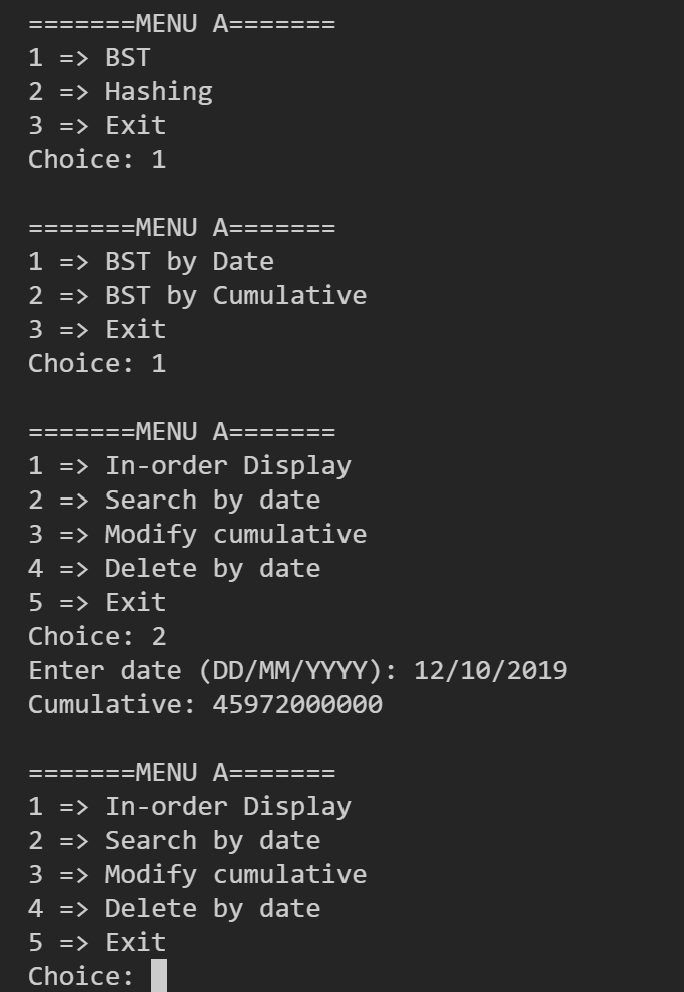
\includegraphics[width=5cm]{scr1.png}
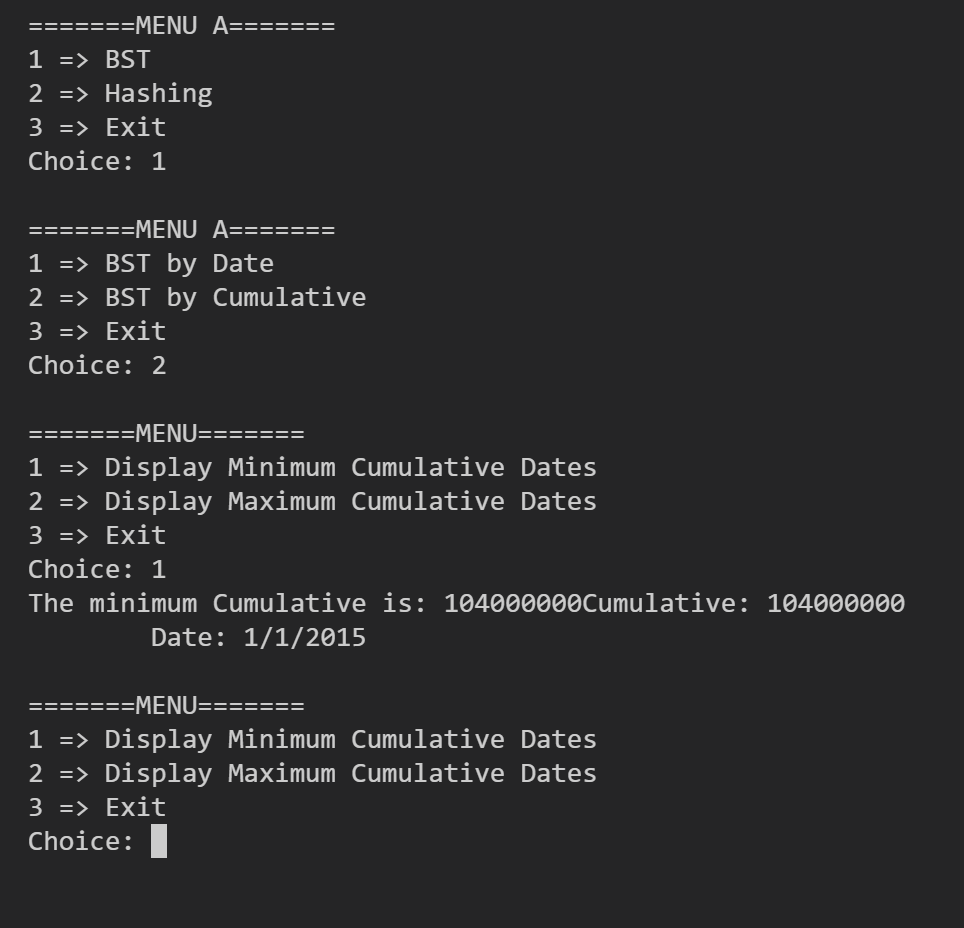
\includegraphics[width=5cm]{scr2.png}
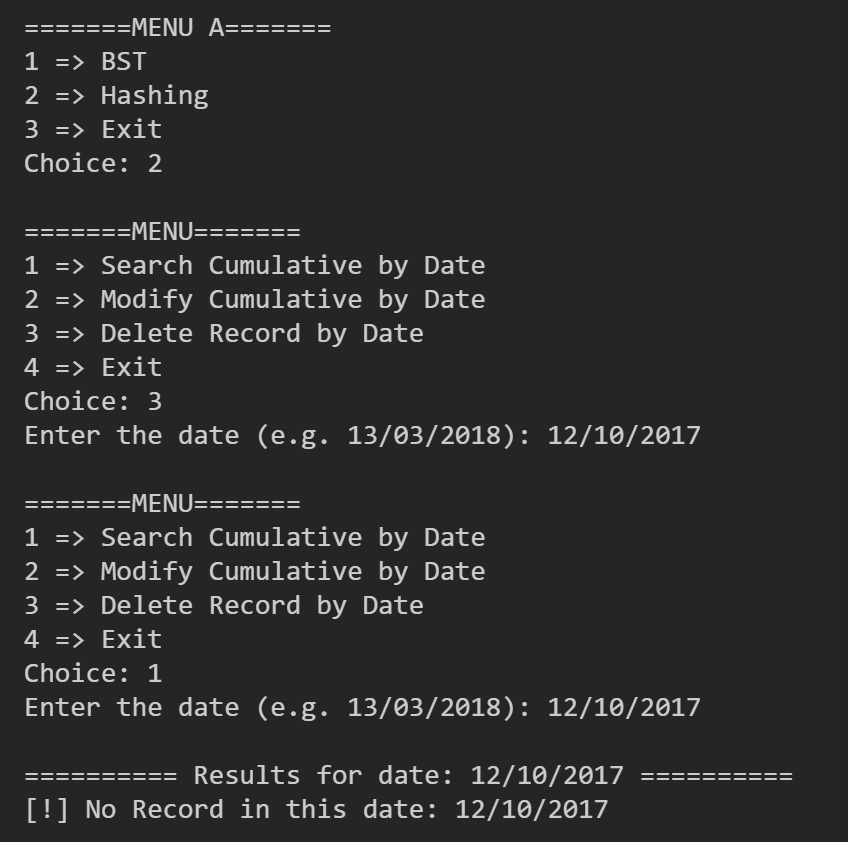
\includegraphics[width=5cm]{scr3.png}
\end{document}